\documentclass[11pt, oneside]{article}   	
\usepackage{geometry}                		
\geometry{letterpaper}                   		
\usepackage{graphicx}				
\usepackage{amssymb}
\usepackage{float}
\usepackage{adjustbox}

\title{Ethnic Fractionalization Using Names}
\author{}
\date{}	

\begin{document}
\maketitle

%\section{Introduction}

%\section{Data}

\section{Methods}

\noindent Features
\begin{itemize}
\item Split names into n-grams using characters
\item Test using all lowercase letters and marking which letters begin and end a name (relevant for naive bayes and SVM, which are order agnostic). Idea here is to basically give algorithm information as to whether n-gram of characters starts a name, ends a name, or is in the middle of a name.
\end{itemize}

\noindent Algorithms
\begin{itemize}
\item NB (Naive Bayes)
\item SVM (Support Vector Machine)
\item NN (Neural Network)
\end{itemize}

\noindent Parameters
\begin{itemize}
\item {\bf Word Case:} Either (1) make all letters lower case, (2) make start and end of words upper case, which adds additional information to the algorithm -- instead of just letters, the algorithm will also know whether group of letters are from beginning, middle or end of name.
\item {\bf ngrams:} N-grams to make out of letters. (For example, with the word ``word'', using an n-gram of 2 would give us: wo, or, rd.).
\item {\bf trim min:} If an n-gram appears in less than $trim~min$ proportion of names, we exclude it. (ie, remove super rare n-grams).
\item {\bf trim max:} If an n-gram appears in more than $trim~max$ proportion of names, we exclude it. (ie, remove super common n-grams).
\end{itemize}

\noindent Accuracy
\begin{itemize}
\item Assess accuracy of predictions as well as accuracy of the predicted Herfindalh index. We randomly assign each observation into groups of size 50. For each group, we compute the actual and predicted Herfindalh Index. Figure \ref{herf_index_dist} shows the distribution of the Herfindalh index across groups using the d10 variable.
\end{itemize}

\begin{figure}[H]
  \caption{Distribution of Herfindahl index of true d10 groups across randomly assigned groups}
  \label{herf_index_dist}
  \centering
    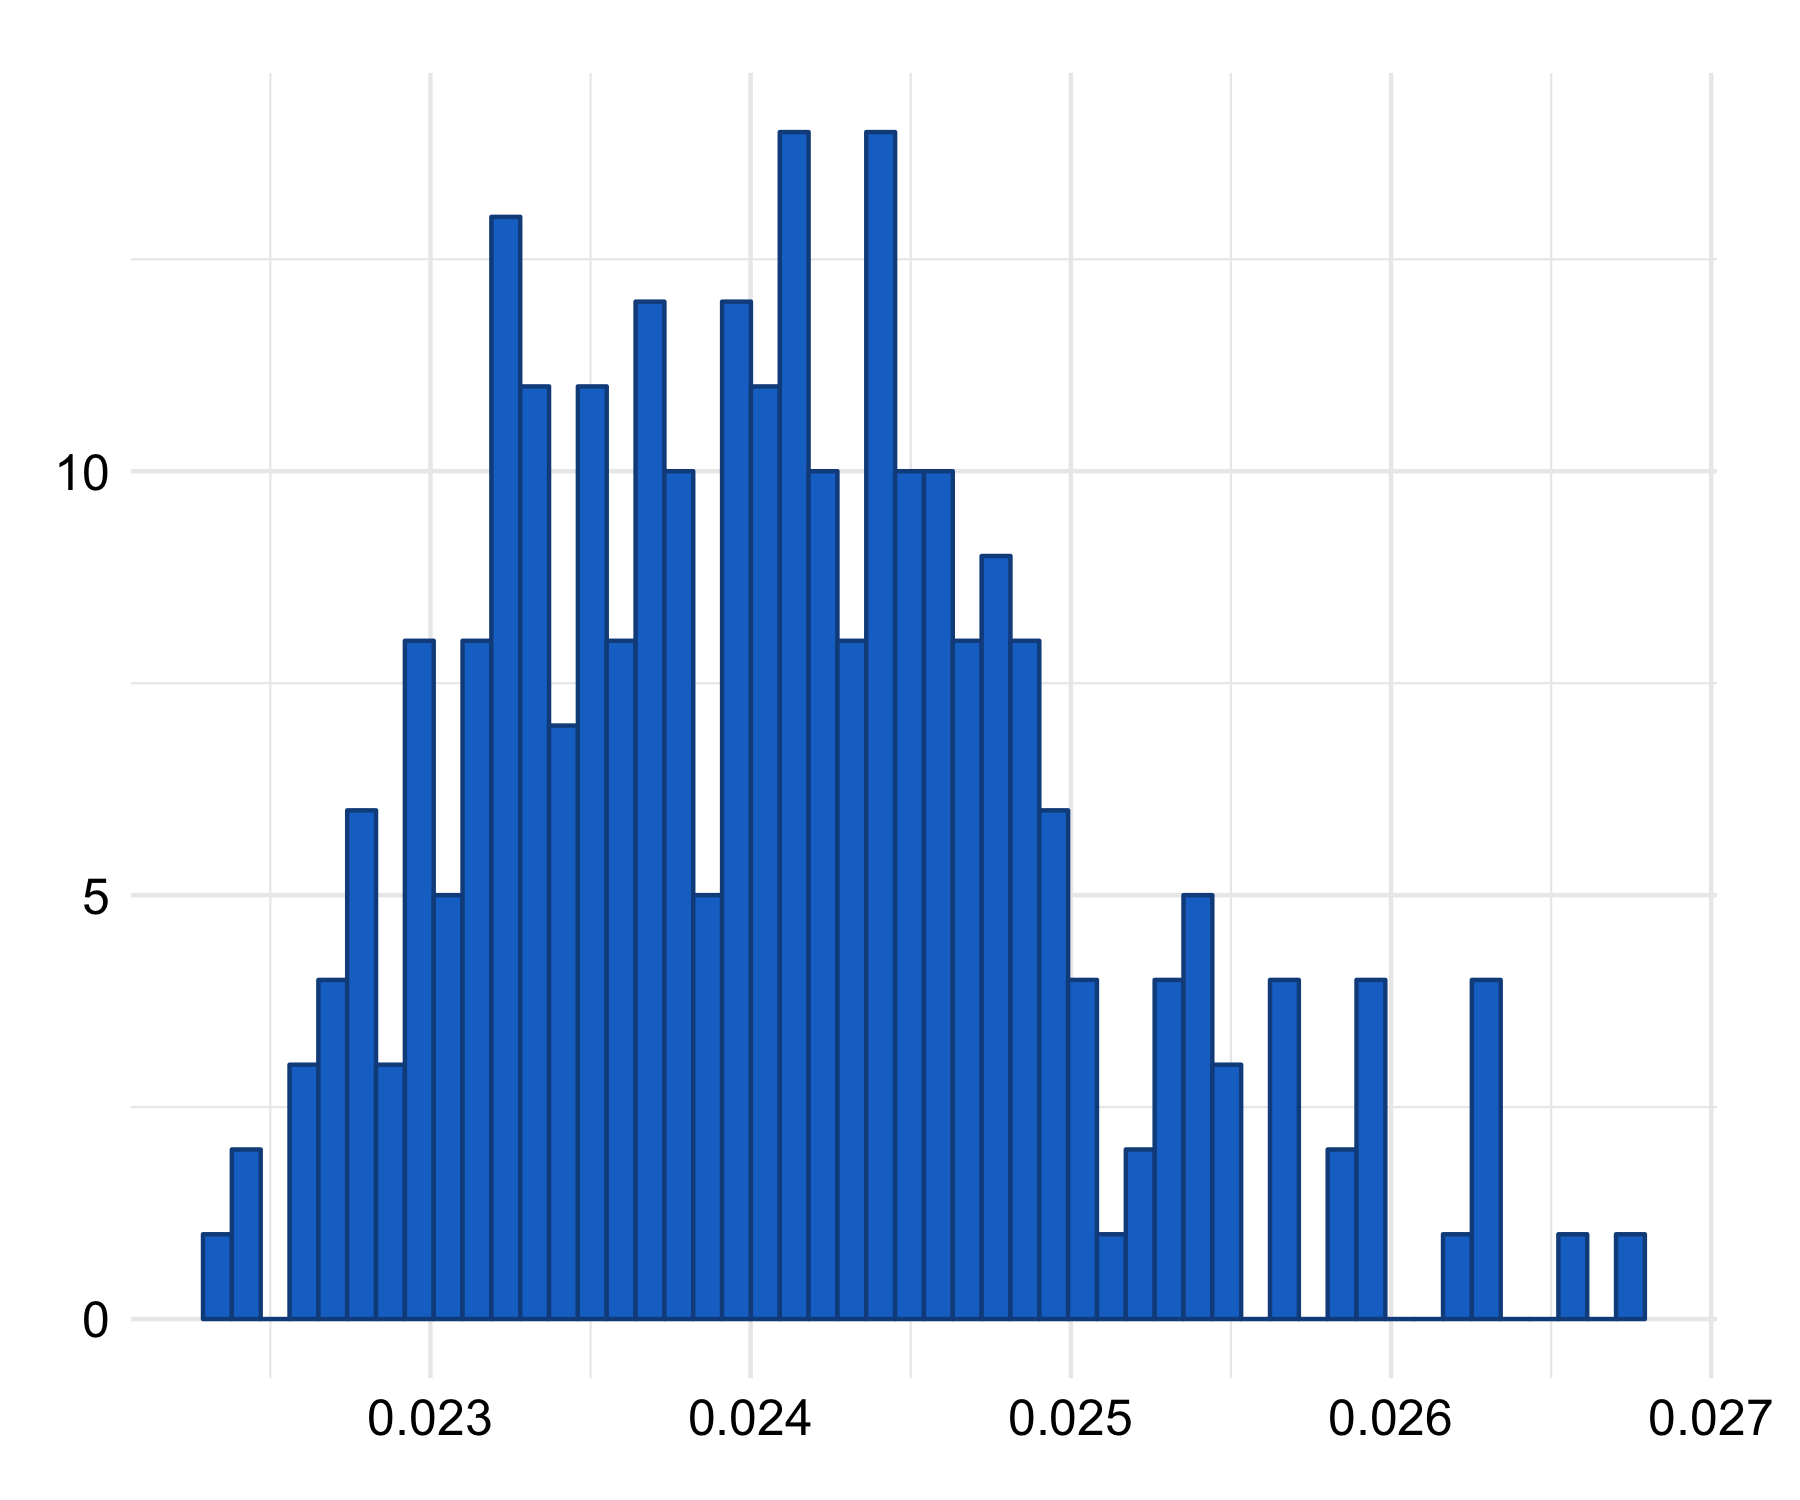
\includegraphics[width=0.7\textwidth]{Figures/herfindalh_truth_index.png}
\end{figure}

\newpage
\section{Results}

Reporting results of both out of sample and in sample tests. Large differences between in sample and out of sample results suggests that the algorithm is overfitting.
\par
For the Herfindahl index, we compute the average absolute difference between the predicted and actual index, and the correlation between the actual and predicted index.

% --------------------------------
\subsection{Religion}

\setlength{\tabcolsep}{10pt}
\begin{table}[H]
\caption{Religion Results: Test Set (Out of Sample)}
\centering
%\begin{adjustbox}{width=1\textwidth}
\begin{tabular}{ccc | cccc} \hline \multicolumn{3}{c |}{Accuracy} & \multicolumn{4}{c}{Parameters} \\ NB & SVM & NN  & Case & ngrams & trim min & trim max \\ \hline 0.9374 & 0.9432 & 0.9368 & lower & 3,4 & 0.001 & 0.9  \\ 0.9391 & 0.9432 & 0.9379 & lower & 2,3,4 & 0.001 & 0.9  \\ 0.9397 & 0.9424 & 0.9356 & lower & 2,3,4,5,6 & 0.001 & 0.9  \\ 0.9409 & 0.9421 & 0.9371 & lower & 2,3,4,5 & 0.001 & 0.9  \\ 0.9394 & 0.9421 & 0.9409 & startend cap & 2,3,4 & 0.001 & 0.9  \\ 0.9397 & 0.9415 & 0.9397 & startend cap & 2,3,4,5 & 0.001 & 0.9  \\ 0.9385 & 0.9409 & 0.9374 & lower & 3,4,5 & 0.001 & 0.9  \\ 0.9388 & 0.9409 & 0.9356 & lower & 3,4,5,6 & 0.001 & 0.9  \\ 0.9391 & 0.9406 & 0.9391 & startend cap & 2,3,4,5,6 & 0.001 & 0.9  \\ 0.9344 & 0.9397 & 0.9356 & startend cap & 2,3 & 0.001 & 0.9  \\ \hline\end{tabular}
%\end{adjustbox}
\end{table}

\setlength{\tabcolsep}{10pt}
\begin{table}[H]
\caption{Religion Results: Train Set (In Sample)}
\centering
%\begin{adjustbox}{width=1\textwidth}
\begin{tabular}{ccc | cccc} \hline \multicolumn{3}{c |}{Accuracy} & \multicolumn{4}{c}{Parameters} \\ NB & SVM & NN  & Case & ngrams & trim min & trim max \\ \hline 0.9482 & 0.9786 & 0.9971 & lower & 3,4 & 0.001 & 0.9  \\ 0.947 & 0.98 & 0.9968 & lower & 2,3,4 & 0.001 & 0.9  \\ 0.9467 & 0.9836 & 0.9969 & lower & 2,3,4,5,6 & 0.001 & 0.9  \\ 0.9465 & 0.9824 & 0.9969 & lower & 2,3,4,5 & 0.001 & 0.9  \\ 0.9481 & 0.981 & 0.9973 & startend cap & 2,3,4 & 0.001 & 0.9  \\ 0.9478 & 0.9838 & 0.9973 & startend cap & 2,3,4,5 & 0.001 & 0.9  \\ 0.9482 & 0.9807 & 0.9966 & lower & 3,4,5 & 0.001 & 0.9  \\ 0.9478 & 0.9818 & 0.9967 & lower & 3,4,5,6 & 0.001 & 0.9  \\ 0.9467 & 0.9838 & 0.9969 & startend cap & 2,3,4,5,6 & 0.001 & 0.9  \\ 0.9451 & 0.9739 & 0.9973 & startend cap & 2,3 & 0.001 & 0.9  \\ \hline\end{tabular}
%\end{adjustbox}
\end{table}

% -------------------------------------------------
\newpage
\subsection{D1}

\setlength{\tabcolsep}{10pt}
\begin{table}[H]
\caption{D1 Results: Test Set (Out of Sample)}
\centering
\begin{adjustbox}{width=1\textwidth}
\begin{tabular}{ccc | ccc | ccc | cccc} \hline \multicolumn{3}{c |}{Accuracy} & \multicolumn{3}{c |}{Avg Diff Herf} & \multicolumn{3}{c |}{Cor. True vs Pred Herf} & \multicolumn{4}{c}{Parameters} \\ NB & SVM & NN &  NB & SVM & NN &  NB & SVM & NN & Case & ngrams & trim min & trim max \\ \hline 0.4176 & 0.9882 & 0.9879 & 0.0039 & 1e-04 & 1e-04 & -0.0499 & 0 & 0.442 & startend cap & 1 & 0.001 & 0.9  \\ 0.7203 & 0.9888 & 0.9879 & 0.0016 & 1e-04 & 1e-04 & 0.1158 & 0.0995 & 0.3525 & startend cap & 2 & 0.001 & 0.9  \\ 0.3112 & 0.9882 & 0.9876 & 0.0031 & 1e-04 & 1e-04 & -0.0182 & 0 & 0.3105 & startend cap & 3 & 0.01 & 0.9  \\ 0.2926 & 0.9882 & 0.9874 & 0.003 & 1e-04 & 1e-04 & 0.0383 & 0 & 0.2959 & startend cap & 3,4 & 0.01 & 0.9  \\ 0.1118 & 0.9882 & 0.9882 & 0.0092 & 1e-04 & 1e-04 & 0.2478 & 0 & 0 & lower & 5 & 0.01 & 0.9  \\ 0.0935 & 0.9882 & 0.9882 & 0.0102 & 1e-04 & 1e-04 & 0.2429 & 0 & 0 & startend cap & 4 & 0.02 & 0.9  \\ 0.2879 & 0.9879 & 0.9871 & 0.0027 & 1e-04 & 1e-04 & 0.0847 & -0.0707 & 0.2417 & startend cap & 3,4,5,6 & 0.01 & 0.9  \\ 0.0821 & 0.9882 & 0.9879 & 0.0096 & 1e-04 & 1e-04 & 0.2371 & 0 & -0.0707 & startend cap & 5 & 0.01 & 0.9  \\ 0.5088 & 0.9891 & 0.9876 & 0.0026 & 1e-04 & 1e-04 & -0.0941 & 0.0519 & 0.2063 & startend cap & 2,3 & 0.01 & 0.9  \\ 0.5215 & 0.9885 & 0.9868 & 0.0027 & 1e-04 & 1e-04 & -0.0274 & -0.036 & 0.2052 & startend cap & 2 & 0.01 & 0.9  \\ \hline\end{tabular}
\end{adjustbox}
\end{table}

\setlength{\tabcolsep}{10pt}
\begin{table}[H]
\caption{D1 Results: Train Set (In Sample)}
\centering
\begin{adjustbox}{width=1\textwidth}
\begin{tabular}{ccc | ccc | ccc | cccc} \hline \multicolumn{3}{c |}{Accuracy} & \multicolumn{3}{c |}{Avg Diff Herf} & \multicolumn{3}{c |}{Cor. True vs Pred Herf} & \multicolumn{4}{c}{Parameters} \\ NB & SVM & NN &  NB & SVM & NN &  NB & SVM & NN & Case & ngrams & trim min & trim max \\ \hline 0.4315 & 0.9856 & 0.9889 & 0.0039 & 1e-04 & 1e-04 & 0.8648 & 0.9958 & 0.9965 & startend cap & 1 & 0.001 & 0.9  \\ 0.7198 & 0.9874 & 0.9987 & 0.0018 & 1e-04 & 0 & 0.929 & 0.9964 & 0.9996 & startend cap & 2 & 0.001 & 0.9  \\ 0.3246 & 0.9857 & 0.9926 & 0.0034 & 1e-04 & 0 & 0.926 & 0.9958 & 0.998 & startend cap & 3 & 0.01 & 0.9  \\ 0.3099 & 0.9864 & 0.9931 & 0.0033 & 1e-04 & 0 & 0.9204 & 0.9961 & 0.9985 & startend cap & 3,4 & 0.01 & 0.9  \\ 0.1167 & 0.9856 & 0.9858 & 0.0094 & 1e-04 & 1e-04 & 0.8884 & 0.9958 & 0.9958 & lower & 5 & 0.01 & 0.9  \\ 0.1022 & 0.9856 & 0.9858 & 0.0102 & 1e-04 & 1e-04 & 0.8975 & 0.9958 & 0.9958 & startend cap & 4 & 0.02 & 0.9  \\ 0.3104 & 0.9864 & 0.9921 & 0.003 & 1e-04 & 1e-04 & 0.9297 & 0.9961 & 0.9981 & startend cap & 3,4,5,6 & 0.01 & 0.9  \\ 0.0914 & 0.9856 & 0.9861 & 0.0097 & 1e-04 & 1e-04 & 0.8983 & 0.9958 & 0.9959 & startend cap & 5 & 0.01 & 0.9  \\ 0.5284 & 0.9875 & 0.9985 & 0.0027 & 1e-04 & 0 & 0.9178 & 0.9965 & 0.9994 & startend cap & 2,3 & 0.01 & 0.9  \\ 0.5414 & 0.9864 & 0.9985 & 0.0028 & 1e-04 & 0 & 0.9167 & 0.9961 & 0.9995 & startend cap & 2 & 0.01 & 0.9  \\ \hline\end{tabular}
\end{adjustbox}
\end{table}

% -------------------------------------------------
\newpage
\subsection{D3}

\setlength{\tabcolsep}{10pt}
\begin{table}[H]
\caption{D3 Results: Test Set (Out of Sample)}
\centering
\begin{adjustbox}{width=1\textwidth}
\begin{tabular}{ccc | ccc | ccc | cccc} \hline \multicolumn{3}{c |}{Accuracy} & \multicolumn{3}{c |}{Avg Diff Herf} & \multicolumn{3}{c |}{Cor. True vs Pred Herf} & \multicolumn{4}{c}{Parameters} \\ NB & SVM & NN &  NB & SVM & NN &  NB & SVM & NN & Case & ngrams & trim min & trim max \\ \hline 0.7247 & 0.9885 & 0.9885 & 0.0016 & 1e-04 & 1e-04 & 0.1692 & 0.1464 & 0.5363 & startend cap & 2 & 0.001 & 0.9  \\ 0.3991 & 0.9882 & 0.9859 & 0.0113 & 1e-04 & 1e-04 & 0.4543 & 0 & 0.2169 & startend cap & 6 & 0.001 & 0.9  \\ 0.4144 & 0.9882 & 0.9859 & 0.0109 & 1e-04 & 1e-04 & 0.4094 & 0 & 0.1907 & lower & 6 & 0.001 & 0.9  \\ 0.2376 & 0.9882 & 0.9871 & 0.0054 & 1e-04 & 1e-04 & -0.0737 & 0 & 0.3569 & startend cap & 3 & 0.01 & 0.9  \\ 0.2121 & 0.9882 & 0.9868 & 0.0054 & 1e-04 & 1e-04 & -0.0683 & 0 & 0.345 & startend cap & 3,4 & 0.01 & 0.9  \\ 0.8271 & 0.9888 & 0.9844 & 7e-04 & 1e-04 & 1e-04 & 0.3294 & 0.1011 & 0.3091 & startend cap & 2,3 & 0.001 & 0.9  \\ 0.4994 & 0.9885 & 0.9853 & 0.0076 & 1e-04 & 1e-04 & 0.295 & 0.2146 & 0.3107 & lower & 5 & 0.001 & 0.9  \\ 0.6385 & 0.9885 & 0.9847 & 0.0025 & 1e-04 & 1e-04 & 0.2904 & 0.2146 & 0.0973 & startend cap & 3,4,5,6 & 0.001 & 0.9  \\ 0.2094 & 0.9882 & 0.9865 & 0.0051 & 1e-04 & 1e-04 & -0.0061 & 0 & 0.2858 & startend cap & 3,4,5,6 & 0.01 & 0.9  \\ 0.2065 & 0.9882 & 0.9868 & 0.0052 & 1e-04 & 1e-04 & 0.0156 & 0 & 0.2857 & startend cap & 3,4,5 & 0.01 & 0.9  \\ \hline\end{tabular}
\end{adjustbox}
\end{table}

\setlength{\tabcolsep}{10pt}
\begin{table}[H]
\caption{D3 Results: Train Set (In Sample)}
\centering
\begin{adjustbox}{width=1\textwidth}
\begin{tabular}{ccc | ccc | ccc | cccc} \hline \multicolumn{3}{c |}{Accuracy} & \multicolumn{3}{c |}{Avg Diff Herf} & \multicolumn{3}{c |}{Cor. True vs Pred Herf} & \multicolumn{4}{c}{Parameters} \\ NB & SVM & NN &  NB & SVM & NN &  NB & SVM & NN & Case & ngrams & trim min & trim max \\ \hline 0.7266 & 0.9875 & 0.9981 & 0.0017 & 1e-04 & 0 & 0.9278 & 0.9975 & 0.9995 & startend cap & 2 & 0.001 & 0.9  \\ 0.4113 & 0.9857 & 0.9909 & 0.0116 & 1e-04 & 1e-04 & 0.6201 & 0.9968 & 0.998 & startend cap & 6 & 0.001 & 0.9  \\ 0.4277 & 0.9859 & 0.9907 & 0.0109 & 1e-04 & 1e-04 & 0.6153 & 0.9968 & 0.9978 & lower & 6 & 0.001 & 0.9  \\ 0.2527 & 0.9858 & 0.9929 & 0.0055 & 1e-04 & 0 & 0.9211 & 0.9968 & 0.9986 & startend cap & 3 & 0.01 & 0.9  \\ 0.2206 & 0.9863 & 0.9929 & 0.0055 & 1e-04 & 0 & 0.8957 & 0.9973 & 0.9987 & startend cap & 3,4 & 0.01 & 0.9  \\ 0.8376 & 0.9916 & 0.9984 & 8e-04 & 1e-04 & 0 & 0.9672 & 0.9979 & 0.9995 & startend cap & 2,3 & 0.001 & 0.9  \\ 0.5162 & 0.9872 & 0.9935 & 0.0074 & 1e-04 & 0 & 0.7724 & 0.9973 & 0.9988 & lower & 5 & 0.001 & 0.9  \\ 0.6592 & 0.9922 & 0.9976 & 0.0023 & 0 & 0 & 0.9153 & 0.9982 & 0.9992 & startend cap & 3,4,5,6 & 0.001 & 0.9  \\ 0.2177 & 0.9864 & 0.9925 & 0.0053 & 1e-04 & 0 & 0.8946 & 0.9973 & 0.9986 & startend cap & 3,4,5,6 & 0.01 & 0.9  \\ 0.2168 & 0.9864 & 0.9929 & 0.0054 & 1e-04 & 0 & 0.8935 & 0.9973 & 0.9985 & startend cap & 3,4,5 & 0.01 & 0.9  \\ \hline\end{tabular}
\end{adjustbox}
\end{table}

% -------------------------------------------------
\newpage
\subsection{D5}

\setlength{\tabcolsep}{10pt}
\begin{table}[H]
\caption{D5 Results: Test Set (Out of Sample)}
\centering
\begin{adjustbox}{width=1\textwidth}
\begin{tabular}{ccc | ccc | ccc | cccc} \hline \multicolumn{3}{c |}{Accuracy} & \multicolumn{3}{c |}{Avg Diff Herf} & \multicolumn{3}{c |}{Cor. True vs Pred Herf} & \multicolumn{4}{c}{Parameters} \\ NB & SVM & NN &  NB & SVM & NN &  NB & SVM & NN & Case & ngrams & trim min & trim max \\ \hline 0.7165 & 0.9885 & 0.9871 & 0.0072 & 0.0038 & 0.0038 & -0.0256 & 0.3261 & 0.0353 & startend cap & 2 & 0.001 & 0.9  \\ 0.4482 & 0.9885 & 0.9865 & 0.0067 & 0.0038 & 0.0037 & -0.2084 & 0.3261 & 0.1899 & startend cap & 2 & 0.01 & 0.9  \\ 0.3224 & 0.9882 & 0.9879 & 0.0057 & 0.0038 & 0.0037 & -0.182 & 0 & 0.2926 & startend cap & 2,3,4 & 0.02 & 0.9  \\ 0.2065 & 0.9879 & 0.9871 & 0.0059 & 0.0038 & 0.0037 & -0.092 & -0.0839 & 0.2446 & startend cap & 3,4,5,6 & 0.01 & 0.9  \\ 0.2118 & 0.9882 & 0.9865 & 0.006 & 0.0038 & 0.0037 & -0.218 & 0 & 0.2155 & startend cap & 3,4 & 0.01 & 0.9  \\ 0.38 & 0.9882 & 0.9871 & 0.006 & 0.0038 & 0.0036 & -0.214 & 0 & 0.2098 & lower & 2,3,4 & 0.02 & 0.9  \\ 0.2076 & 0.9879 & 0.9868 & 0.006 & 0.0038 & 0.0036 & -0.1634 & -0.0839 & 0.2045 & startend cap & 3,4,5 & 0.01 & 0.9  \\ 0.2335 & 0.9882 & 0.9879 & 0.0061 & 0.0038 & 0.0036 & -0.1213 & 0 & 0.1956 & startend cap & 3 & 0.01 & 0.9  \\ 0.3682 & 0.9882 & 0.9868 & 0.0061 & 0.0038 & 0.0037 & -0.2114 & 0 & 0.1939 & lower & 2,3 & 0.02 & 0.9  \\ 0.0026 & 0.9882 & 0.9882 & 0.013 & 0.0038 & 0.0038 & 0.1729 & 0 & 0 & lower & 5 & 0.02 & 0.9  \\ \hline\end{tabular}
\end{adjustbox}
\end{table}

\setlength{\tabcolsep}{10pt}
\begin{table}[H]
\caption{D5 Results: Train Set (In Sample)}
\centering
\begin{adjustbox}{width=1\textwidth}
\begin{tabular}{ccc | ccc | ccc | cccc} \hline \multicolumn{3}{c |}{Accuracy} & \multicolumn{3}{c |}{Avg Diff Herf} & \multicolumn{3}{c |}{Cor. True vs Pred Herf} & \multicolumn{4}{c}{Parameters} \\ NB & SVM & NN &  NB & SVM & NN &  NB & SVM & NN & Case & ngrams & trim min & trim max \\ \hline 0.7217 & 0.9876 & 0.9981 & 0.0081 & 0.0016 & 6e-04 & 0.5595 & 0.5813 & 0.941 & startend cap & 2 & 0.001 & 0.9  \\ 0.4691 & 0.9864 & 0.9983 & 0.007 & 0.0015 & 5e-04 & 0.481 & 0.5815 & 0.9614 & startend cap & 2 & 0.01 & 0.9  \\ 0.3348 & 0.9863 & 0.9969 & 0.0052 & 0.0015 & 6e-04 & 0.5154 & 0.5802 & 0.9148 & startend cap & 2,3,4 & 0.02 & 0.9  \\ 0.2178 & 0.9865 & 0.9921 & 0.0057 & 0.0015 & 0.0018 & 0.4573 & 0.5862 & 0.7257 & startend cap & 3,4,5,6 & 0.01 & 0.9  \\ 0.2239 & 0.9864 & 0.9926 & 0.0057 & 0.0015 & 0.002 & 0.4556 & 0.5766 & 0.7386 & startend cap & 3,4 & 0.01 & 0.9  \\ 0.3956 & 0.987 & 0.997 & 0.0058 & 0.0014 & 6e-04 & 0.5135 & 0.6056 & 0.911 & lower & 2,3,4 & 0.02 & 0.9  \\ 0.2184 & 0.9865 & 0.9922 & 0.0057 & 0.0015 & 0.0025 & 0.4516 & 0.5862 & 0.6933 & startend cap & 3,4,5 & 0.01 & 0.9  \\ 0.2499 & 0.9859 & 0.9932 & 0.0059 & 0.0016 & 0.0021 & 0.4132 & 0.5528 & 0.7477 & startend cap & 3 & 0.01 & 0.9  \\ 0.3847 & 0.9867 & 0.9983 & 0.006 & 0.0014 & 5e-04 & 0.4999 & 0.6028 & 0.954 & lower & 2,3 & 0.02 & 0.9  \\ 0.0064 & 0.9856 & 0.9856 & 0.015 & 0.0016 & 0.0016 & 0.4596 & 0.5483 & 0.5483 & lower & 5 & 0.02 & 0.9  \\ \hline\end{tabular}
\end{adjustbox}
\end{table}

% -------------------------------------------------
\newpage
\subsection{D7}

\setlength{\tabcolsep}{10pt}
\begin{table}[H]
\caption{D7 Results: Test Set (Out of Sample)}
\centering
\begin{adjustbox}{width=1\textwidth}
\begin{tabular}{ccc | ccc | ccc | cccc} \hline \multicolumn{3}{c |}{Accuracy} & \multicolumn{3}{c |}{Avg Diff Herf} & \multicolumn{3}{c |}{Cor. True vs Pred Herf} & \multicolumn{4}{c}{Parameters} \\ NB & SVM & NN &  NB & SVM & NN &  NB & SVM & NN & Case & ngrams & trim min & trim max \\ \hline 0.4482 & 0.9885 & 0.9871 & 0.0039 & 3e-04 & 3e-04 & -0.2888 & 0.153 & 0.313 & startend cap & 2 & 0.01 & 0.9  \\ 0.4956 & 0.9882 & 0.9844 & 0.0034 & 3e-04 & 3e-04 & -0.2314 & 0 & 0.2889 & lower & 2,3 & 0.01 & 0.9  \\ 0.8426 & 0.9885 & 0.9868 & 0.0011 & 3e-04 & 3e-04 & -0.0231 & -0.0362 & 0.2751 & lower & 2,3 & 0.001 & 0.9  \\ 0.2335 & 0.9882 & 0.9865 & 0.0052 & 3e-04 & 3e-04 & 0.0597 & 0 & 0.2556 & startend cap & 3 & 0.01 & 0.9  \\ 0.2718 & 0.9882 & 0.9879 & 0.0051 & 3e-04 & 3e-04 & -0.0775 & 0 & 0.2377 & lower & 3 & 0.01 & 0.9  \\ 0.2065 & 0.9879 & 0.9871 & 0.0052 & 3e-04 & 3e-04 & 0.084 & -0.0825 & 0.2329 & startend cap & 3,4,5,6 & 0.01 & 0.9  \\ 0.8197 & 0.9882 & 0.9874 & 0.0017 & 3e-04 & 3e-04 & 0.1978 & 0 & 0.2195 & startend cap & 2,3 & 0.001 & 0.9  \\ 0.2118 & 0.9882 & 0.9865 & 0.0052 & 3e-04 & 3e-04 & 0.0489 & 0 & 0.2061 & startend cap & 3,4 & 0.01 & 0.9  \\ 0.5229 & 0.9885 & 0.9871 & 0.0032 & 3e-04 & 3e-04 & -0.1073 & 0.1138 & 0.2061 & lower & 2,3,4 & 0.01 & 0.9  \\ 0.0291 & 0.9882 & 0.9882 & 0.0194 & 3e-04 & 3e-04 & 0.2044 & 0 & 0 & lower & 6 & 0.01 & 0.9  \\ \hline\end{tabular}
\end{adjustbox}
\end{table}

\setlength{\tabcolsep}{10pt}
\begin{table}[H]
\caption{D7 Results: Train Set (In Sample)}
\centering
\begin{adjustbox}{width=1\textwidth}
\begin{tabular}{ccc | ccc | ccc | cccc} \hline \multicolumn{3}{c |}{Accuracy} & \multicolumn{3}{c |}{Avg Diff Herf} & \multicolumn{3}{c |}{Cor. True vs Pred Herf} & \multicolumn{4}{c}{Parameters} \\ NB & SVM & NN &  NB & SVM & NN &  NB & SVM & NN & Case & ngrams & trim min & trim max \\ \hline 0.4691 & 0.9864 & 0.9981 & 0.0039 & 2e-04 & 1e-04 & 0.9267 & 0.976 & 0.9944 & startend cap & 2 & 0.01 & 0.9  \\ 0.5092 & 0.9876 & 0.9978 & 0.0036 & 2e-04 & 1e-04 & 0.9394 & 0.9772 & 0.9937 & lower & 2,3 & 0.01 & 0.9  \\ 0.8535 & 0.9908 & 0.9985 & 0.0018 & 2e-04 & 1e-04 & 0.9034 & 0.982 & 0.9941 & lower & 2,3 & 0.001 & 0.9  \\ 0.2499 & 0.9859 & 0.9931 & 0.0052 & 2e-04 & 1e-04 & 0.8707 & 0.9743 & 0.9868 & startend cap & 3 & 0.01 & 0.9  \\ 0.2856 & 0.9864 & 0.995 & 0.0051 & 2e-04 & 1e-04 & 0.8901 & 0.9717 & 0.9883 & lower & 3 & 0.01 & 0.9  \\ 0.2178 & 0.9865 & 0.9924 & 0.0053 & 2e-04 & 1e-04 & 0.8668 & 0.9765 & 0.9874 & startend cap & 3,4,5,6 & 0.01 & 0.9  \\ 0.8288 & 0.9915 & 0.9984 & 0.002 & 2e-04 & 1e-04 & 0.9177 & 0.9837 & 0.994 & startend cap & 2,3 & 0.001 & 0.9  \\ 0.2239 & 0.9864 & 0.993 & 0.0053 & 2e-04 & 1e-04 & 0.8679 & 0.976 & 0.9877 & startend cap & 3,4 & 0.01 & 0.9  \\ 0.5325 & 0.988 & 0.9982 & 0.0034 & 2e-04 & 1e-04 & 0.9369 & 0.9778 & 0.9936 & lower & 2,3,4 & 0.01 & 0.9  \\ 0.0312 & 0.9856 & 0.9857 & 0.0202 & 2e-04 & 2e-04 & 0.7833 & 0.9741 & 0.9742 & lower & 6 & 0.01 & 0.9  \\ \hline\end{tabular}
\end{adjustbox}
\end{table}

% -------------------------------------------------
\newpage
\subsection{D10}

\setlength{\tabcolsep}{10pt}
\begin{table}[H]
\caption{D10 Results: Test Set (Out of Sample)}
\centering
\begin{adjustbox}{width=1\textwidth}
\begin{tabular}{ccc | ccc | ccc | cccc} \hline \multicolumn{3}{c |}{Accuracy} & \multicolumn{3}{c |}{Avg Diff Herf} & \multicolumn{3}{c |}{Cor. True vs Pred Herf} & \multicolumn{4}{c}{Parameters} \\ NB & SVM & NN &  NB & SVM & NN &  NB & SVM & NN & Case & ngrams & trim min & trim max \\ \hline 0.2609 & 0.4968 & 0.4597 & 0.0027 & 0.0021 & 0.0012 & 0.1868 & 0.2868 & 0.5892 & lower & 2,3,4 & 0.001 & 0.9  \\ 0.2432 & 0.4824 & 0.4741 & 0.0018 & 0.0025 & 0.0016 & 0.2615 & 0.3 & 0.4822 & lower & 3 & 0.001 & 0.9  \\ 0.2426 & 0.4868 & 0.4518 & 0.0024 & 0.002 & 0.0015 & 0.3359 & 0.3213 & 0.4787 & startend cap & 3,4,5 & 0.001 & 0.9  \\ 0.2406 & 0.4844 & 0.4612 & 0.0023 & 0.0025 & 0.0016 & 0.2708 & 0.4749 & 0.4641 & startend cap & 3 & 0.001 & 0.9  \\ 0.2588 & 0.4885 & 0.4591 & 0.0027 & 0.0018 & 0.0013 & 0.2049 & 0.4002 & 0.4717 & lower & 2,3,4,5,6 & 0.001 & 0.9  \\ 0.2465 & 0.4891 & 0.4826 & 0.0024 & 0.0022 & 0.0014 & 0.2942 & 0.4615 & 0.452 & startend cap & 2,3 & 0.001 & 0.9  \\ 0.2524 & 0.4976 & 0.4547 & 0.0024 & 0.0022 & 0.0015 & 0.3371 & 0.3019 & 0.426 & lower & 3,4 & 0.001 & 0.9  \\ 0.1109 & 0.4441 & 0.4574 & 0.0019 & 0.0033 & 0.0026 & 0.0783 & 0.422 & 0.2541 & lower & 2,3 & 0.02 & 0.9  \\ 0.1391 & 0.4462 & 0.465 & 0.0019 & 0.003 & 0.0022 & 0.0952 & 0.1826 & 0.4173 & lower & 2 & 0.001 & 0.9  \\ 0.0697 & 0.42 & 0.4365 & 0.0036 & 0.0041 & 0.0039 & 0.2596 & 0.0978 & 0.4107 & lower & 3 & 0.02 & 0.9  \\ \hline\end{tabular}
\end{adjustbox}
\end{table}

\setlength{\tabcolsep}{10pt}
\begin{table}[H]
\caption{D10 Results: Train Set (In Sample)}
\centering
\begin{adjustbox}{width=1\textwidth}
\begin{tabular}{ccc | ccc | ccc | cccc} \hline \multicolumn{3}{c |}{Accuracy} & \multicolumn{3}{c |}{Avg Diff Herf} & \multicolumn{3}{c |}{Cor. True vs Pred Herf} & \multicolumn{4}{c}{Parameters} \\ NB & SVM & NN &  NB & SVM & NN &  NB & SVM & NN & Case & ngrams & trim min & trim max \\ \hline 0.3657 & 0.7787 & 0.9509 & 0.0029 & 0.0011 & 3e-04 & 0.8598 & 0.9639 & 0.9934 & lower & 2,3,4 & 0.001 & 0.9  \\ 0.3493 & 0.6548 & 0.9338 & 0.0022 & 0.0017 & 4e-04 & 0.8822 & 0.9322 & 0.9928 & lower & 3 & 0.001 & 0.9  \\ 0.3703 & 0.7894 & 0.954 & 0.0022 & 0.0011 & 2e-04 & 0.8313 & 0.9598 & 0.9945 & startend cap & 3,4,5 & 0.001 & 0.9  \\ 0.3604 & 0.6717 & 0.9409 & 0.0022 & 0.0013 & 3e-04 & 0.8594 & 0.9269 & 0.9921 & startend cap & 3 & 0.001 & 0.9  \\ 0.37 & 0.8266 & 0.9526 & 0.0034 & 9e-04 & 3e-04 & 0.793 & 0.9718 & 0.9936 & lower & 2,3,4,5,6 & 0.001 & 0.9  \\ 0.3434 & 0.7216 & 0.9484 & 0.0025 & 0.0013 & 3e-04 & 0.8476 & 0.9439 & 0.9933 & startend cap & 2,3 & 0.001 & 0.9  \\ 0.3754 & 0.7573 & 0.95 & 0.0021 & 0.0012 & 3e-04 & 0.873 & 0.9577 & 0.9937 & lower & 3,4 & 0.001 & 0.9  \\ 0.1399 & 0.4823 & 0.7444 & 0.0023 & 0.0027 & 0.0012 & 0.8238 & 0.8755 & 0.9495 & lower & 2,3 & 0.02 & 0.9  \\ 0.1886 & 0.498 & 0.7879 & 0.0017 & 0.0025 & 9e-04 & 0.8556 & 0.8736 & 0.9624 & lower & 2 & 0.001 & 0.9  \\ 0.0831 & 0.4218 & 0.4937 & 0.0038 & 0.0035 & 0.0031 & 0.7583 & 0.8708 & 0.8841 & lower & 3 & 0.02 & 0.9  \\ \hline\end{tabular}
\end{adjustbox}
\end{table}

% -------------------------------------------------
\newpage
\subsection{Ethnicity}

\setlength{\tabcolsep}{10pt}
\begin{table}[H]
\caption{Ethnicity Results: Test Set (Out of Sample)}
\centering
\begin{adjustbox}{width=1\textwidth}
\begin{tabular}{ccc | ccc | ccc | cccc} \hline \multicolumn{3}{c |}{Accuracy} & \multicolumn{3}{c |}{Avg Diff Herf} & \multicolumn{3}{c |}{Cor. True vs Pred Herf} & \multicolumn{4}{c}{Parameters} \\ NB & SVM & NN &  NB & SVM & NN &  NB & SVM & NN & Case & ngrams & trim min & trim max \\ \hline 0.2309 & 0.3665 & 0.3468 & 0.0015 & 0.0018 & 0.0019 & 0.0085 & 0.4445 & 0.5091 & lower & 2,3,4 & 0.001 & 0.9  \\ 0.2379 & 0.3618 & 0.345 & 0.0015 & 0.0015 & 0.0016 & 0.1139 & 0.5028 & 0.3117 & startend cap & 2,3,4,5 & 0.001 & 0.9  \\ 0.2326 & 0.3574 & 0.3456 & 0.0015 & 0.0017 & 0.0015 & 0.0571 & 0.4983 & 0.494 & lower & 2,3,4,5 & 0.001 & 0.9  \\ 0.2374 & 0.3712 & 0.3459 & 0.0015 & 0.0016 & 0.0015 & 0.1144 & 0.4349 & 0.4633 & startend cap & 2,3,4 & 0.001 & 0.9  \\ 0.2382 & 0.3609 & 0.3432 & 0.0017 & 0.0018 & 0.0016 & 0.0925 & 0.4451 & 0.4308 & startend cap & 2,3,4,5,6 & 0.001 & 0.9  \\ 0.2171 & 0.3641 & 0.3494 & 0.0016 & 0.0015 & 0.0017 & -0.0137 & 0.4437 & 0.4102 & startend cap & 3 & 0.001 & 0.9  \\ 0.2315 & 0.3568 & 0.3382 & 0.0015 & 0.0018 & 0.0017 & 0.0702 & 0.4121 & 0.4401 & lower & 2,3,4,5,6 & 0.001 & 0.9  \\ 0.115 & 0.3035 & 0.3253 & 0.0018 & 0.0022 & 0.002 & 0.083 & 0.2092 & 0.4307 & startend cap & 2,3 & 0.01 & 0.9  \\ 0.2224 & 0.3626 & 0.3582 & 0.0016 & 0.0017 & 0.0017 & 0.0806 & 0.426 & 0.3884 & startend cap & 2,3 & 0.001 & 0.9  \\ 0.2182 & 0.3582 & 0.34 & 0.0018 & 0.0018 & 0.0015 & 0.0172 & 0.4222 & 0.3667 & lower & 3,4,5 & 0.001 & 0.9  \\ \hline\end{tabular}
\end{adjustbox}
\end{table}

\setlength{\tabcolsep}{10pt}
\begin{table}[H]
\caption{Ethnicity Results: Train Set (In Sample)}
\centering
\begin{adjustbox}{width=1\textwidth}
\begin{tabular}{ccc | ccc | ccc | cccc} \hline \multicolumn{3}{c |}{Accuracy} & \multicolumn{3}{c |}{Avg Diff Herf} & \multicolumn{3}{c |}{Cor. True vs Pred Herf} & \multicolumn{4}{c}{Parameters} \\ NB & SVM & NN &  NB & SVM & NN &  NB & SVM & NN & Case & ngrams & trim min & trim max \\ \hline 0.3784 & 0.7769 & 0.936 & 0.0016 & 6e-04 & 3e-04 & 0.7915 & 0.9543 & 0.9852 & lower & 2,3,4 & 0.001 & 0.9  \\ 0.3874 & 0.8274 & 0.9434 & 0.0018 & 5e-04 & 3e-04 & 0.779 & 0.964 & 0.9878 & startend cap & 2,3,4,5 & 0.001 & 0.9  \\ 0.3822 & 0.8208 & 0.9377 & 0.0016 & 5e-04 & 3e-04 & 0.7871 & 0.9602 & 0.9856 & lower & 2,3,4,5 & 0.001 & 0.9  \\ 0.3856 & 0.7932 & 0.9412 & 0.0017 & 6e-04 & 3e-04 & 0.7973 & 0.9594 & 0.9853 & startend cap & 2,3,4 & 0.001 & 0.9  \\ 0.3829 & 0.8462 & 0.9462 & 0.0018 & 4e-04 & 3e-04 & 0.7795 & 0.9636 & 0.988 & startend cap & 2,3,4,5,6 & 0.001 & 0.9  \\ 0.3728 & 0.6324 & 0.914 & 0.0018 & 8e-04 & 4e-04 & 0.8176 & 0.9138 & 0.9788 & startend cap & 3 & 0.001 & 0.9  \\ 0.3805 & 0.8392 & 0.939 & 0.0019 & 5e-04 & 3e-04 & 0.7642 & 0.9627 & 0.9879 & lower & 2,3,4,5,6 & 0.001 & 0.9  \\ 0.1886 & 0.4733 & 0.7759 & 0.0024 & 0.0013 & 6e-04 & 0.7629 & 0.8817 & 0.9446 & startend cap & 2,3 & 0.01 & 0.9  \\ 0.36 & 0.6974 & 0.928 & 0.0019 & 7e-04 & 3e-04 & 0.7712 & 0.9318 & 0.9872 & startend cap & 2,3 & 0.001 & 0.9  \\ 0.3876 & 0.7991 & 0.9379 & 0.002 & 5e-04 & 3e-04 & 0.7941 & 0.9583 & 0.9865 & lower & 3,4,5 & 0.001 & 0.9  \\ \hline\end{tabular}
\end{adjustbox}
\end{table}

%\section{}
%\subsection{}

\end{document} 



 